\maketitle
\tableofcontents
\newpage

\section{Zielsetzung}
Ziel dieses Versuches ist es, gedämpfte und erzwungene Schwingungen zu untersuchen.
\section{Theorie}
Ein Schwingkreis besteht in seiner einfachsten Form aus einem Kondensator mit der Kapzität
$C$ und einer Spule mit der Induktivität $L$. Die Energie in diesem Schwingkreis oszilliert
zwischen den beiden Energiespeichern und hat als mögliche Maxima ein maximales magnetisches
Feld in der Spule und einen maximal aufgeladenen Kondensator. Falls ein idealer Draht
vorliegt, wird diese $\textbf{ungedämpfte Schwingung}$ für $t \to \infty$ unverändert schwingen.
\begin{figure}
  \centering
  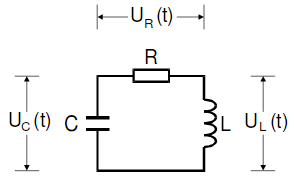
\includegraphics[scale=0.6]{gSchwingkreis.png}
  \caption{Schaltbild eines gedämpften Schwingkreises \cite{anleitung}.}
  \label{fig:1}
\end{figure}

Falls nun aber ein endlicher Widerstand $R$ in den Schaltkreis eingebaut wird, siehe \ref{fig:1},
dann wird ein Teil der elektrischen Energie an diesem ohmschen Widerstand in Wärme umgewandelt.
Damit fallen die Amplituden der Spannung und des Stromes mit der Zeit ab und es entwickelt sich
eine $\textbf{gedämpften Schwingung}$.

\section{Durchführung}

\subsection{Versuchsaufbau}

\subsection{Versuchsdurchführung}
\section{Auswertung}

\section{Diskussion}
\newpage
\nocite{*}
\printbibliography
